\chapter{INTRODUÇÃO}

Este trabalho visa apresentar as experiencias vividas durante o período como estagiário do o LEMAF (Laboratório de Projetos e Estudos
em Manejo Florestal), laboratório situado dentro da Universidade Federal de Lavras(UFLA) onde são desenvolvidas soluções tecnológicas relacionadas a manejo florestal.
O laboratório foi inaugurado em 2002 e desde lá, vem desenvolvimento diversos projetos para diversos órgãos e empresas, contando em 2018 com mais de 100 funcionários.

\begin{figure}[H]
\centering
\caption{Convenção Lemaf / Fundecc 2018} %legenda
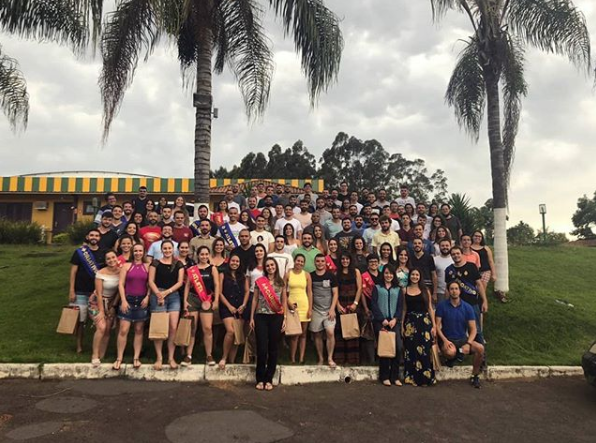
\includegraphics[scale=1]{convensao}\\  % o 0.9 indica 90% do tamanho original
% pdfLaTeX aceita figuras no formato PNG, JPG ou PDF
% figuras vetoriais podem ser exportadas para eps e depois convertidas para pdf usando epstopdf
{\small Fonte: https://www.instagram.com/p/Brlf2IKlAmi/} %Fonte da imagem
\label{fig:exemplo} %rotulo para refencia
\end{figure}

Os projetos do LEMAF são no geral ligados ao meio ambiente, como monitoramento de áreas desmatadas e uso indevido de recursos hídricos, porém seu arsenal de projetos inclui diversos temas, como portais para povos indigenas, monitoramento de numero de animais atropelados por região e ate mesmo gerenciadores de conteudos.   
O estágio proporcionado pelo mesmo tinha como responsabilidades o seguimento de metodologias ágeis, organização e trabalho em equipe e principalmente o desenvolvimento de projetos web.

Por conta de uma grande rotação de projetos e times, foi necessário o estudo de diversos frameworks e tecnologias, onde os principais relacionados com frontend foram Angular, Vuejs e ReactJs, enquanto com backend foram SpringBoot, DotNet Framework e PlayFramework.
Para que o desenvolvimento dos projetos fluíssem efetivamente, eram utilizadas diversas metodologias ágeis, como principais Scrum e Kambam.

Com toda essa carga de conhecimento e responsabilidades ser estagiario no LEMAF se tornou uma experiencia incrivel, uma vez que não era tratado como tal. Estava sempre evoluindo, conhecendo novas tecnologias do mercado e tendo oportunidade de obter conhecimento de pessoas extremamente experientes no ramo.